\documentclass[aps,pra,onecolumn, superscriptaddress]{revtex4}
\usepackage{graphicx}
\usepackage{natbib}
\usepackage{hyperref} 
\usepackage{mathtools}

% \documentclass[letterpaper,10pt]{article}
% \usepackage{natbib}
% \usepackage{osameet2}
% \usepackage{hyperref}  

%% standard packages and arguments should be modified as needed

\usepackage{amsmath,amssymb}

% \usepackage[pdftex,colorlinks=true,bookmarks=false,citecolor=blue,urlcolor=blue]{hyperref} %pdflatex
% \usepackage[dvips,colorlinks=true,bookmarks=false,citecolor=blue,urlcolor=blue]{hyperref} %latex w/dvips 

\begin{document}
\section{Experimental Setup}
      
% Following Ho et al.~\cite{Ho2009}, we denote the detection times recorded by Alice's (Bob's) local clock by $t\,(t')$.
In general, Alice and Bob's clocks are not synchronized.
With $t$ local time at Alice's, and $ t'$ local time at Bob's,
we define the time offset $\delta = t' - t$.
% When Alice and Bob's clock are located together detecting the same event, the difference between the detection times measured by their local clocks would be $\delta = t' - t$.
We use the time correlation of photon pairs generated in SPDC to determine $\delta$.
% We first conduct an experiment to determine this offset, under the controlled condition that the two clocks run at the same frequency. 
% We will lift this constraint in our future work by applying the algorithm described in~\cite{Ho2009}.

\begin{figure}[htbp]
  \centering
  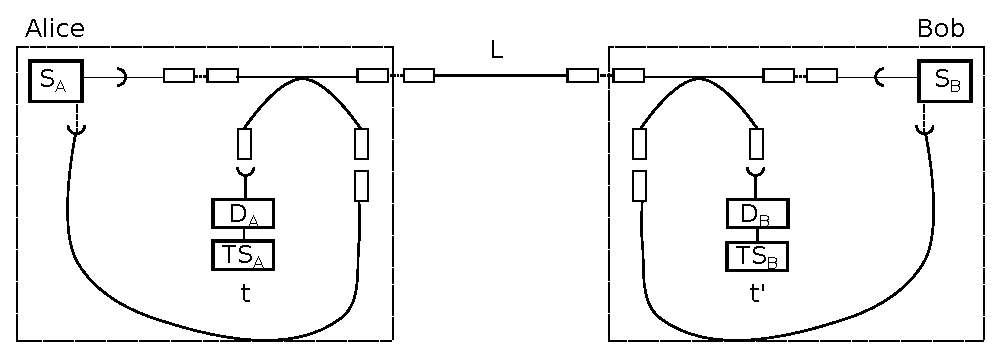
\includegraphics[width=16cm]{figures/setup_simplified.eps}
  \caption{\label{fig:setup}
  Time synchronization setup. Alice and Bob each have a source of time-correlated photon pairs produced by spontaneous paramateric down-conversion (SPDC) and a single photon detector. One member of the SPDC pair is detected locally at detector $D_A$ on Alice's side and at $D_B$ on Bob's side. The other member of the pair is sent through a single mode fibre to be detected on the remote side. Times of arrival for all detected photons are recorded in each lab with respect to a local clock. 
  }
\end{figure}

A sketch of the experimental setup is shown in Figure~\ref{fig:setup}.
The system is symmetrical: both Alice and Bob generate time-correlated photon pairs (810 nm) using collinear type-II SPDC.
Fibre beam splitters route the vertically polarized photons to local measurements, while the orthogonal component travels and is detected at the remote location.

Photons are detected using avalanche photodiodes (Perkin Elmer C30902SH, measured jitter time of 495 \textbf{error!} ps).
Detection events at each location are timestamped with temporal resolution 125~ps.
% are time-stamped with individual timestamp units (temporal resolution of 125 ps). The absolute time recorded by each unit is derived by adding the elapsed time to the unix time evaluated upon the starting of the timestamp unit. 

% Both timestamp units are seeded with a common frequency reference in the form of a rubidium oscillator.

% The unix time differences of Alice’s and Bob’s computers, and the time difference between the unix time evaluation and the start of the timestamp unit at each computer, both contribute to the clock offset $\delta$ between Alice and Bob.
The cross correlation between the Alice's and Bob's event records shows two peaks.   The time separation between peaks corresponds to twice the propagation time between the sources, the midpoint instead is the offset $\delta$ between the clocks.

% To determine the time difference between the clocks, consider a photon pair produced at Alice's site. With finite probability, one photon of the pair is detected locally $D_A$ at time $t$, while the other propagates for $t_L$ over distance $L$ and detected at $D_B$ at time $t'$. The time difference between the time labels for any pair produced at Alice will be: 
% \begin{equation}
% t'-t=t_L + \delta
% \end{equation}

% Similarly for any pair produced at Bob's site:
% \begin{equation}
% t-t'=t_L - \delta
% \end{equation}

% To extract these time differences, we perform a cross correlation between the events on both sides. 
% To efficiently perform this cross correlation, we apply the algorithm described in~\cite{Ho2009}.

\begin{figure}[htbp]
  \centering
  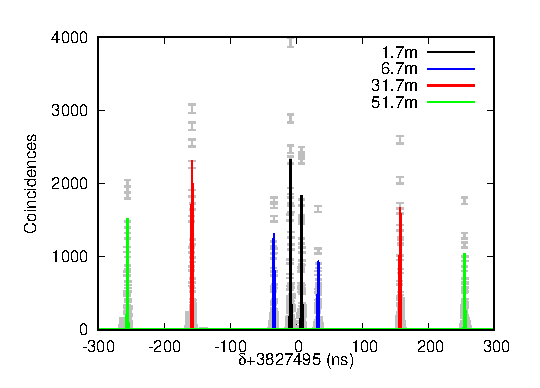
\includegraphics[width=16cm]{figures/g2/g2.eps}
  \caption{\label{fig:g2}
  Timing correlations of Alice and Bob's pair sources measured for various spatial separations $L$ between them.  
  For every $L$, a correlation measurement yields two coincidence peaks, 
  one corresponding to each source.
  The time separation between peaks corresponds to twice the propagation time between the sources, the midpoint instead is the offset between the clocks.
  Solid line: Gaussian fit used to estimate the central position of each peak.
  Error bars: Poissonian standard deviation.
  }
\end{figure}

We repeated the experiment for different length $L$ of fiber connecting A and B locations.
% For every value of $L$, we expect to observe two correlation peaks, one corresponding to each source.
% The left peak $t' - t = \delta - t_L$ (corresponds to pairs originating at Bob) and 
% the right peak $t' - t = \delta + t_L$ (corresponds to pairs originating at Alice).
% An estimate of $\delta$ can thus be derived directly from the mean of the peak positions. 
Figure~\ref{fig:g2} shows four sets of correlation peak pairs obtained for different $L$.

% To determine the peak position with a resolution better than that of the timestamp unit, we accumulate ~2000 data points for each peak distribution and fit it to a gaussian function. 

In table~\ref{table:offsets}, we show that the timing offset $\delta$ estimated for various values of $L$ are in good agreement with each other.

\begin{table}[htbp] 
\centering
\label{table:offsets}
\begin{tabular}{cclll}
$L(m)$ & $\delta + 3827495(ns)$\\
 1.7 & $0.39\pm0.03$\\
 6.7 & $0.44\pm0.03$ \\
 31.7 & $0.37\pm0.03$\\
 51.7 & $0.38\pm0.03$
\end{tabular}
\caption{Estimated clock offset $\delta$ between Alice and Bob's clocks for various spatial separations $L$.}
\end{table}

In this experiment, we seeded both timestamps with a common frequency reference from a rubidium oscillator so that the offset between the two clocks does not drift over the duration of the measurement.
We will lift this constraint in our future work by applying the algorithm already described in~\cite{Ho2009}.
\bibliography{references}     

\end{document}